\section{Chapter 2\\Multi-armed Bandits}


\begin{frame}{The 10-armed Testbed}
\begin{columns}

    \begin{column}{0.5\textwidth}
    \begin{block}{Experimental setup}
    \begin{itemize}[label=$\rightarrow$]
        \item 2000 randomly generated 10-arm bandits
        \item $q_*(a) \sim \mathcal{N}(0,1)$
        \item $R(a) \sim \mathcal{}(q_*(a),1)$
    \end{itemize}
    \end{block}
    \end{column}

    \begin{column}{0.5\textwidth}
        \centering
        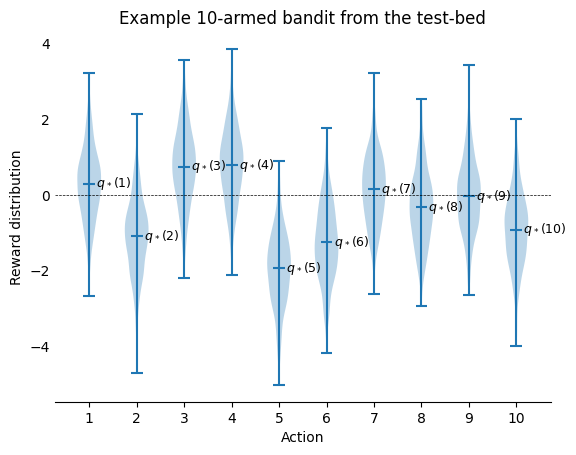
\includegraphics[width=\textwidth]{figures/fig2-1.png}
    \end{column}

\end{columns}
\end{frame}


\begin{frame}{$\epsilon$-greedy agent}
\begin{columns}

    \begin{column}{0.5\textwidth}
    \begin{block}{Experiment}
    \begin{itemize}[label=$\rightarrow$]
        \item $\epsilon$-greedy agent
        \item sample average value estimator
        \item reward at each step averaged over 2000 bandits
    \end{itemize}
    \end{block}
    \end{column}

    \begin{column}{0.5\textwidth}
        \centering
        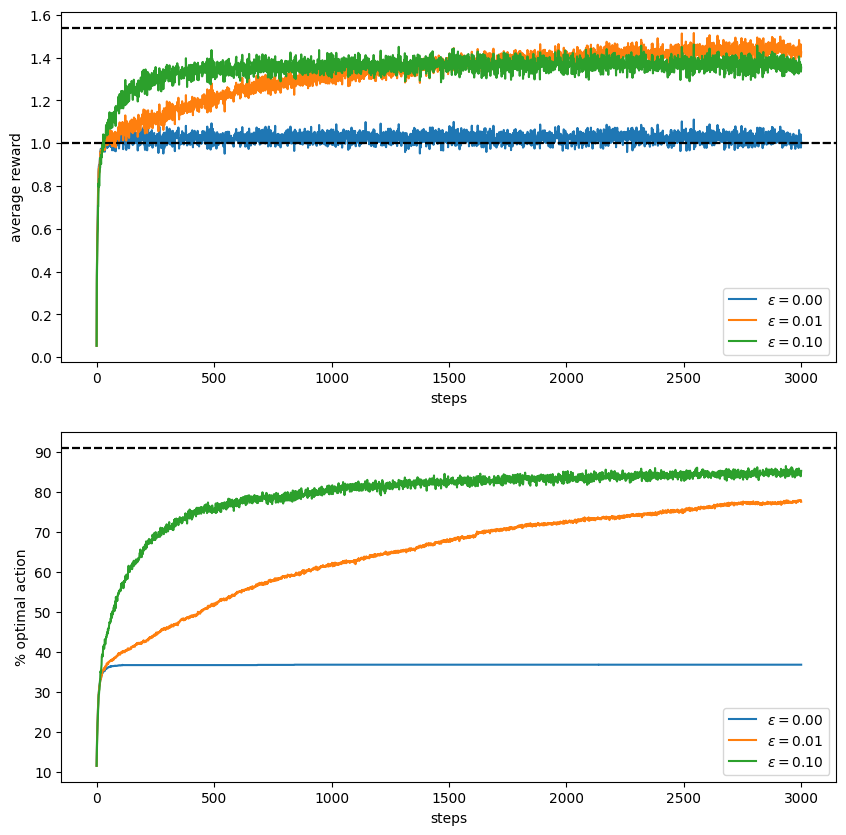
\includegraphics[width=\textwidth]{figures/fig2-2.png}
    \end{column}

\end{columns}
\end{frame}


\begin{frame}{$\epsilon$-greedy agent}
\begin{columns}

    \begin{column}{0.5\textwidth}
        \begin{block}{Observation 1:}
        For $\epsilon=0$, average reward $\approx 1$
        \end{block}
        \begin{block}{What gives?}
            \footnotesize
            \begin{itemize}[label=$\rightarrow$]
                \item This is the expected value of the first positive reward received.
                \item Can be estimated via integrals weighted by survival functions - the chance that a random walk stays positive forever.
                \item Depends on initial action value estimates ($0$ here).
                \item Value is linear in the variance of the expected reward over actions.
            \end{itemize}
        \end{block}
    \end{column}

    \begin{column}{0.5\textwidth}
        \centering
        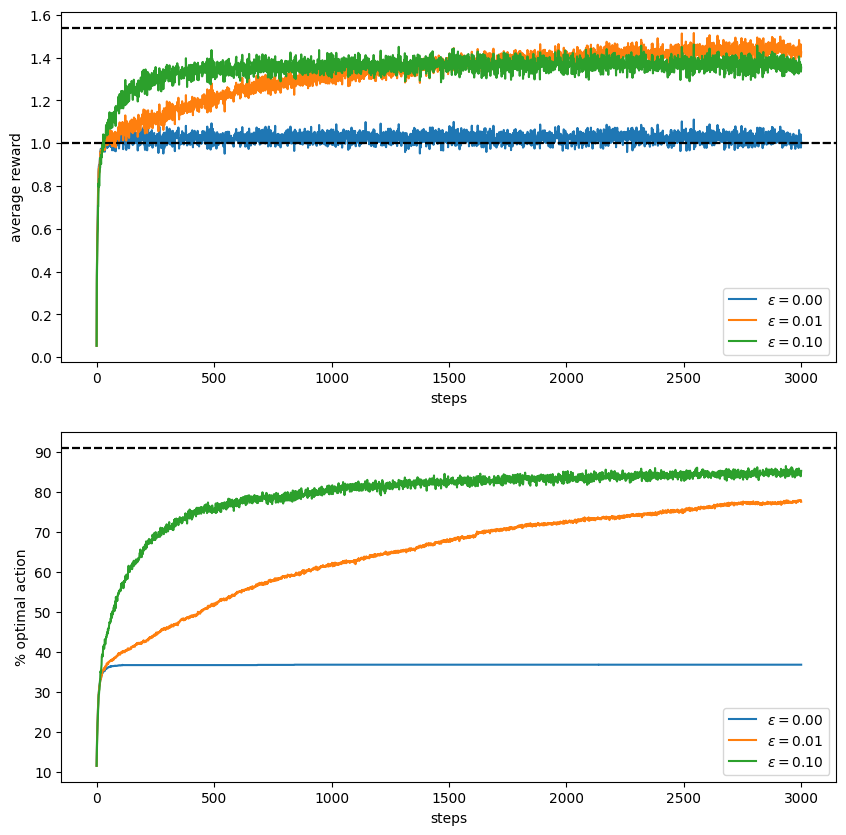
\includegraphics[width=\textwidth]{figures/fig2-2.png}
    \end{column}

\end{columns}
\end{frame}


\begin{frame}{$\epsilon$-greedy agent}
\begin{columns}

    \begin{column}{0.5\textwidth}
        \begin{block}{Observation 2:}
        Average reward $\lesssim 1.54$
        \end{block}
        \begin{block}{What gives?}
            \footnotesize
            \begin{itemize}[label=$\rightarrow$]
                \item Theoretical ceiling, as provided by an oracle agent.
                \item This is the best \textbf{any} agent can do.
                \item Calculated as the expected value of the highest of $k$ action values.
                \item Ceiling $\approx \sqrt{2 \ln k}$
                \item For $k=10$, this ceiling $\approx 1.539$.
            \end{itemize}
        \end{block}
    
    \end{column}
    \begin{column}{0.5\textwidth}
        \centering
        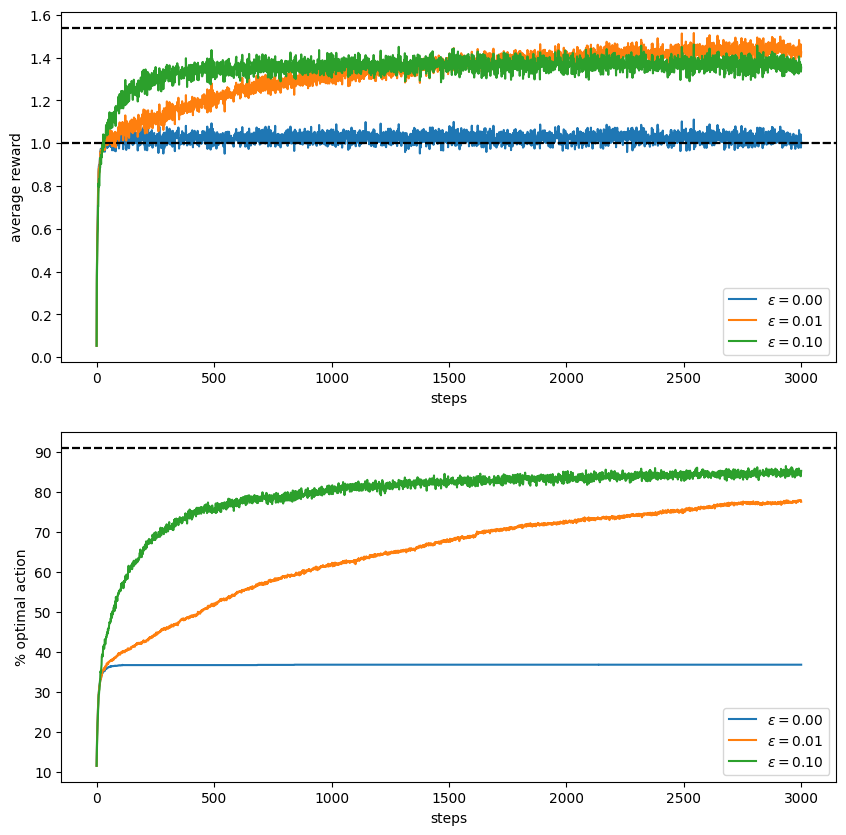
\includegraphics[width=\textwidth]{figures/fig2-2.png}
    \end{column}

\end{columns}
\end{frame}

